\section{Literature Review}
\label{sec:lit-review}

\subsection{The Elliptic Partial Differential Equation}

Partial differential equations are classified by their highest order derivative terms. A second order, linear differential equation can be written as
\begin{align*}
    A(\textbf{x}) \frac{\partial^2 u(\textbf{x})}{\partial x^2} + B(\textbf{x}) \frac{\partial^2 u(\textbf{x})}{\partial x \partial y} + C(\textbf{x}) \frac{\partial^2 u(\textbf{x})}{\partial y^2} + ... \\
    ... + D(\textbf{x}) \frac{\partial u(\textbf{x})}{\partial x} + E(\textbf{x}) \frac{\partial u(\textbf{x})}{\partial y} + F(\textbf{x}) u(\textbf{x}) + G(\textbf{x}) &= 0.
\end{align*}
Second-order linear PDEs are classified according to the value of the determinant of this expression:
\begin{align*}
    B^2 - 4AC &< 0,\ \ \ \text{Elliptic} \\
    B^2 - 4AC &= 0,\ \ \ \text{Parabolic} \\
    B^2 - 4AC &> 0,\ \ \ \text{Hyperbolic}
\end{align*}

In this overview, we will consider common elliptic PDEs such as the Poisson equation
\begin{align}
    \nabla \cdot \left( \beta(\textbf{x}) \nabla u(\textbf{x}) \right) &= f(\textbf{x}),
    \label{eq:variable_poisson}
\end{align}
and the Helmholtz equation
\begin{align}
    \nabla \cdot \left( \beta(\textbf{x}) \nabla u(\textbf{x}) \right) + \lambda(\textbf{x}) u(\textbf{x}) &= f(\textbf{x}),
    \label{eq:variable_helmholtz}
\end{align}
where $\textbf{x} = [x, y]$, $\nabla = (\frac{\partial}{\partial x}, \frac{\partial}{\partial y})$, $\nabla^2 = \nabla \cdot \nabla = \frac{\partial^2}{\partial x^2} + \frac{\partial^2}{\partial y^2}$, and $\textbf{x} \in \Omega \subset \mathcal{R}^2$. When $\beta(\textbf{x}) = 0$ and $\lambda(\textbf{x}) = \kappa^2$ ($\kappa$ is a constant), these expressions reduce to the more classical, constant coefficient versions of the Poisson and Helmholtz equations. When the right-hand side function $f(\textbf{x}) = 0$, these are homogeneous problems, where \refeqn{eq:variable_poisson} is reduced to the Laplace equation. Each of these PDEs are subject to the appropriate boundary conditions on the domain boundary $\partial \Omega = \Gamma$. Such boundary conditions (BCs) can either be Dirichlet (Type-I), Neumann (Type-II), or Robin/Mixed (Type-III) BCs. Dirichlet problems impose the value of $u$ on the boundaries, Neumann problems impose the flux or normal gradient $\partial_n u$ on the boundaries, while Robin problems impose a linear combination of Dirichlet and Neumann type BCs.

Although analytical solutions exist for some simple variations of the problems above, we are interested in looking at numerical methods to solve these equations. To do so, we look at various ways to discretize the domain $\Omega$. This discretization will lead to a linear system of equations which we will solve with numerical methods, taking advantage of the sparsity and structure of the associated system.

\subsection{Numerical Methods for Elliptic PDEs}
\label{sec:numerical-methods-for-elliptic-pdes}

\subsubsection{Finite Difference}
\label{subsub:finite-difference}

\begin{figure}
    \centering
    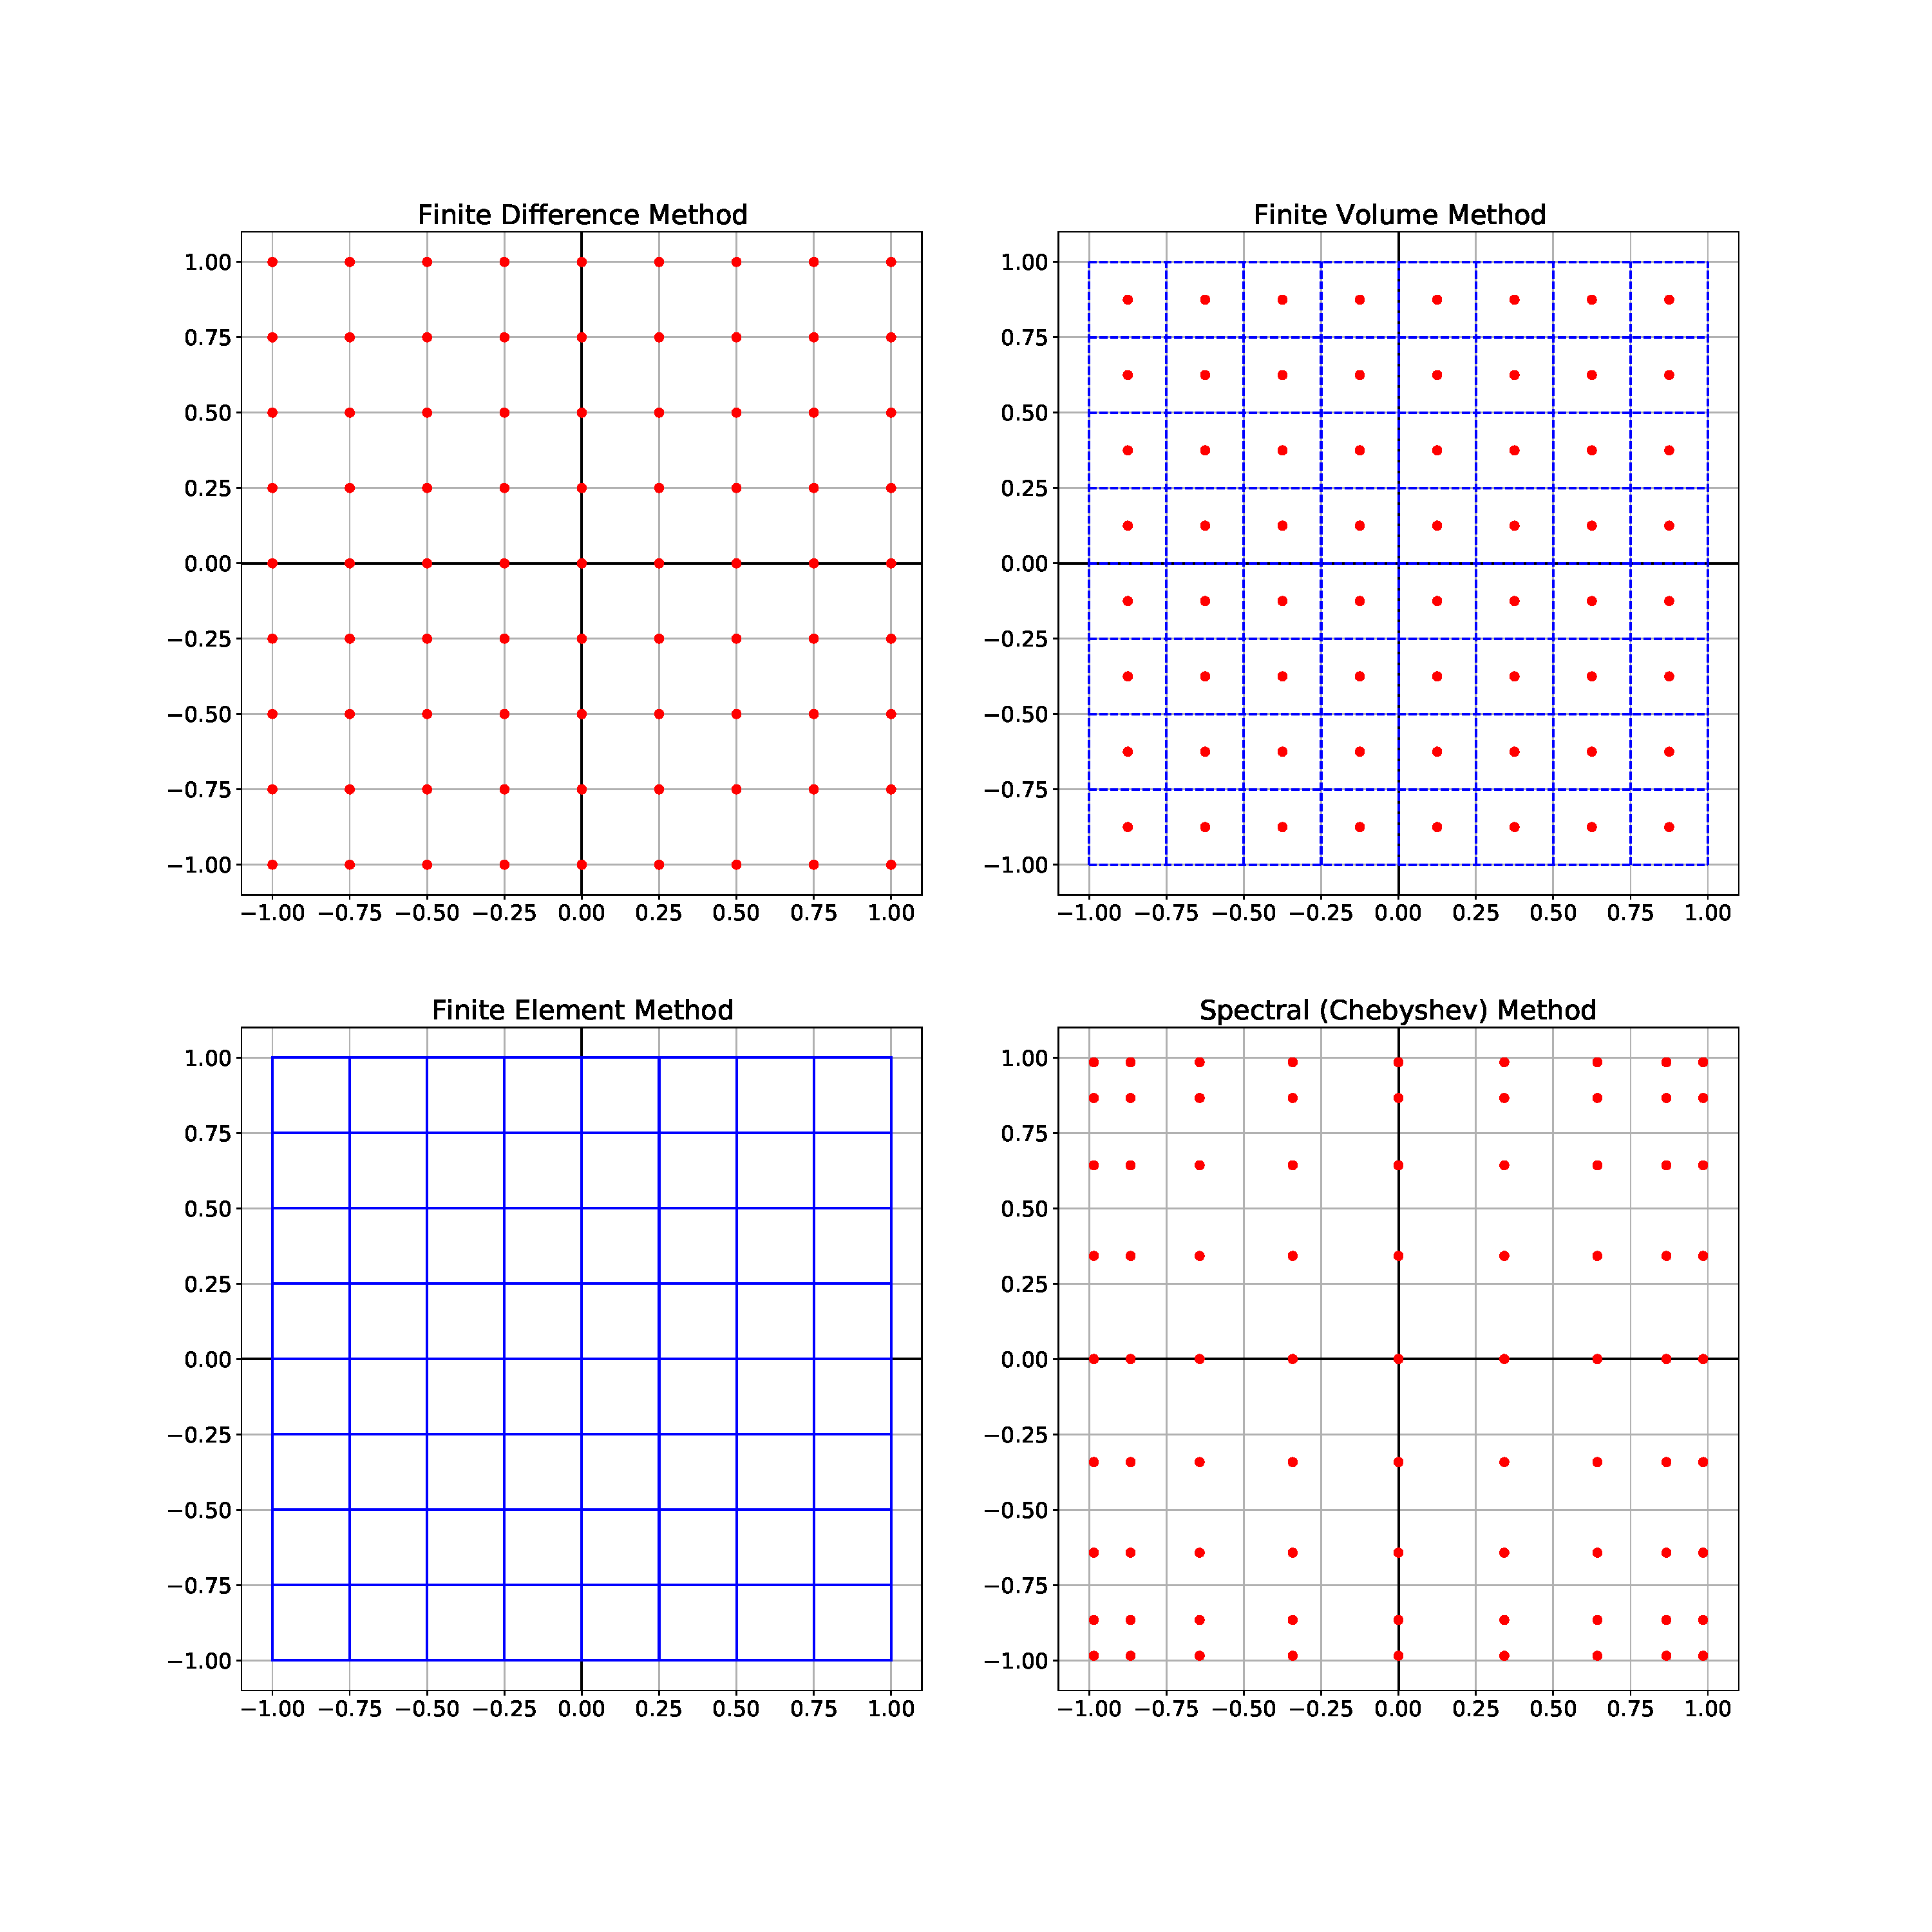
\includegraphics[width=0.8\columnwidth]{figures/PDE_discretization_methods.pdf}
    \caption{Discretization Methods. Top Left: Finite difference grid based on a mesh of points or nodes. Top Right: Finite volume mesh made of cells (dashed blue boxes) with cell averages in the center (red points). Bottom Left: Finite element mesh where each blue box is an element with a shape function defined at all points within the element. Bottom Right: Spectral mesh made up of a tensor of Chebyshev nodes.}
    \label{fig:discretization_methods}
\end{figure}

If $\Omega$ is on a logically rectangular domain (i.e. 2D Cartesian plane), perhaps the simplest discretization of the domain $\Omega$ is by collocating a mesh of points throughout the domain. Given upper and lower bounds in both directions, $[x_l, x_u], [y_l, y_u]$, the x- and y-location of each point can be defined as
\begin{align}
    x_i &= x_l + i \Delta x,\ \ \ i = 0, 1, ..., N_x-1 \\
    y_i &= y_l + j \Delta y,\ \ \ j = 0, 1, ..., N_y-1
\end{align}
where $N_x, N_y$ is the number of points in the x- and y-direction and grid spacing is defined as
\begin{align}
    \Delta x &= \frac{x_u - x_l}{N_x - 1} \\
    \Delta y &= \frac{y_u - y_l}{N_y - 1}.
\end{align}
These points are shown in the first plot of Figure \ref{fig:discretization_methods}. This type of discretization is known as the {\em finite difference method}. In the finite difference approach, the expressions for the derivatives in a PDE are replaced with Taylor series approximations. For example, a second order accurate, central-difference approximation to the second derivative can be given as
\begin{align}
    \frac{\partial^2 u}{\partial x^2} &= \frac{u(x - \Delta x, y) - 2u(x, y) + u(x + \Delta x, y)}{\Delta x^2} + \mathcal{O}(\Delta x^2)
\end{align}
and if we let $u(x_i, y_j) = u_{i,j}$, then we can write this as
\begin{align}
    \frac{\partial^2 u}{\partial x^2} &= \frac{u_{i-1,j} - 2u_{i,j} + u_{i+1,j}}{\Delta x^2} + \mathcal{O}(\Delta x^2).
\end{align}
Using these Taylor Series expansions (and $\beta(x,y) = 1$), we can replace \refeqn{eq:variable_poisson} with the discrete system of equations:
\begin{align}
    \frac{u_{i-1,j} - 2u_{i,j} + u_{i+1,j}}{\Delta x^2} + \frac{u_{i,j-1} - 2u_{i,j} + u_{i,j+1}}{\Delta y^2} &= f_{i,j}.
    \label{eq:poisson_FD}
\end{align}
For each grid point $i = 0, ..., N_x - 1$, $j = 0, ..., N_y - 1$ this expression forms a linear system with $(N_x-1) \times (N_y-1)$ unknowns. The system that is formed from this discretization is sparse and banded. For example, let $N_x = N_y = N$ for simplicity (thus $\Delta x = \Delta y = h$). Index the vector $\textbf{u}$ first by rows, then by columns, such that
\begin{align}
    \textbf{u} = [u_{0,0}, ..., u_{N - 1, 0}, u_{0, 1}, ..., u_{N - 1, 1}, ..., u_{0, N - 1}, ..., u_{N - 1, N - 1}]^T.
\end{align}
The corresponding linear system from \ref{eq:poisson_FD} is the following:
\begin{align}
    \textbf{A} &= \frac{1}{h^2}
    \begin{bmatrix}
        \textbf{D} & \textbf{I}_{N} & \textbf{0} & ... & \textbf{0} \\
        \textbf{I}_{N} & \textbf{D} & \textbf{I}_{N} & ... & \textbf{0} \\
        \textbf{0} & \textbf{I}_{N} & \textbf{D} & ... & \textbf{0} \\
        \vdots & \vdots & \vdots & \ddots & \vdots \\
        \textbf{0} & \textbf{0} & \textbf{0} & ... & \textbf{D}
    \end{bmatrix}
\end{align}
where
\begin{align}
    \textbf{D} &= 
    \begin{bmatrix}
        -4 & 1 & 0 & ... & 0 \\
        1 & -4 & 1 & ... & 0 \\
        0 & 1 & -4 & ... & 0 \\
        \vdots & \vdots & \vdots & \ddots & \vdots \\
        0 & 0 & 0 & ... & -4
    \end{bmatrix}.
\end{align}
We also index the RHS similarly to $u(x,y)$ resulting in a RHS vector $\textbf{f}$. This leads to the linear system
\begin{align}
    \textbf{A} \textbf{u} = \textbf{f} + \textbf{b}
\end{align}
where $\textbf{b}$ contains any updates necessary for any type of boundary condition \citep{leveque2007finite}.

\subsubsection{Finite Volume}

In a finite volume scheme, the domain is broken up into cells, which can be structured or unstructured polygons (2D) or polyhedrons (3D). The function to approximate is solved for in terms of a cell average. Finite volume schemes are often used to solve equations modeling conservation laws, where the cell quantity is conserved in time through balancing fluxes (what comes in and out of the cell boundaries) and the cell source (what the cell is generating or destroying).

Elliptic systems like the Poisson equation can be solved via the finite volume method by considering that the flux across a cell domain can be related to the quantity being advected (Fick's Law). Start with the general, linear conservation law,
\begin{align}
    \frac{\partial q(x,y,t)}{\partial t} + \nabla \cdot \textbf{F}(x,y,t) = s(x,y,t),
\end{align}
and let the flux $\textbf{F}(x,y,t)$ be related to gradient of the quantity: $\textbf{F} = \beta \nabla q$. Plugging this into the conservation equation above yields
\begin{align}
    \frac{\partial q(x,y,t)}{\partial t} + \nabla \cdot \left( \beta(x,y) \nabla q(x,y,t) \right) = s(x,y,t).
\end{align}
For the finite volume method, we integrate over the cell domain $\Omega_i$
\begin{align}
    \frac{\partial}{\partial t} \int_{\Omega_i} q(x,y,t) d\Omega_i + \int_{\Omega_i} \nabla \cdot \left( \beta(x,y) \nabla q(x,y,t) \right) d\Omega_i = \int_{\Omega_i} s(x,y,t) d\Omega_i
\end{align}
and use the divergence theorem to relate the volume integral of the flux to the surface integral of the surface:
\begin{align}
    \frac{\partial}{\partial t} \int_{\Omega_i} q(x,y,t) d\Omega_i + \int_{\Gamma_i} \beta(x,y) \nabla q(x,y,t) \cdot \hat{n}\ d\Gamma_i = \int_{\Omega_i} s(x,y,t) d\Omega_i.
\end{align}
Now, if we only consider the constant coefficient, steady-state case ($\frac{\partial q}{\partial t} = 0$), then we get
\begin{align}
    \int_{\Gamma_i} \nabla q(x,y) \cdot \hat{n}\ d\Gamma_i = \int_{\Omega_i} s(x,y) d\Omega_i.
\end{align}

Discretizing the gradient using neighboring points and evaluating the integrals through cell-centered, averaged values yields a stencil discretization nearly identical to that of finite difference approaches. Special care must be taken at the physical boundaries to enforce Dirichlet or Neumann boundary conditions appropriately. Finite volume approaches that result in a stencil discretization are also sometimes called cell-centered finite difference schemes. These are particularly useful when enforcing Neumann boundary conditions through the use of ghost cells (also called halo cells) \citep{leveque2007finite}.

\subsubsection{Finite Element}

In a finite element scheme, the domain is broken into elements. These elements can also be structured or unstructured polygons (2D) or polyhedrons (3D), similar to the finite volume method. The PDE to solve is converted into a weak form by multiplying the PDE by a test function $v(x,y)$ and integrating over the domain:
\begin{align}
    \int_{\Omega} v \nabla^2 u d\Omega &= \int_{\Omega} vf d\Omega.
\end{align}
Green's Theorem (i.e., integration by parts) is used to break the LHS into integrals on the domain $\Omega$ and the boundary $\partial \Omega = \Gamma$:
\begin{align}
    -\int_{\Omega} \nabla v \cdot \nabla u d\Omega + \int_{\Gamma} v \frac{\partial u}{\partial n} d\Gamma &= \int_{\Omega} vf d\Omega
    \label{eq:poisson_weak_form}
\end{align}
The idea behind the finite element method is to use basis functions
\begin{align}
    u(x,y) \approx \bar{u} = \sum_{k=1}^{N_k} c_k \phi(x,y)
\end{align}
inside each element $\Omega_i$, where $\Omega = \cup_{i = 1}^{N_{\text{elem}}} \Omega_i$. When the same basis functions for the test functions $v$ are also used, this leads to the Galerkin finite element method. Upon substitution of the above into \ref{eq:poisson_weak_form}, and integrating the basis function with either quadrature or with analytical expressions, a linear system is formed for the coefficients $c_k$. This process is referred to as matrix assembly and can be done for local elements or global elements \citep{giraldo2020introduction}.

There are several variations of the finite element method. Depending on the space from which the test functions $v$ are from, one can arrive at the continuous finite element method or the discontinuous finite element method. When $v$ and $u$ are built up with the same basis function (the Galerkin principle), this leads to the Galerkin finite element method \citep{thomee2007galerkin}. By choosing certain shape or basis functions, one can derive different variations of the finite element method, including the B-spline finite element method \citep{kagan1998new} and the spectral element method \citep{patera1984spectral}.

\subsubsection{Spectral Methods}

In spectral methods, the approach is to approximate the solution $u$ as a linear combination of a finite set of orthogonal basis functions
\begin{align}
    u(x,y) = \sum_{i=1}^{N_x} \sum_{j=1}^{N_y} c_{i,j} \phi_{i}(x) \phi_{j}(y)
\end{align}
where the coefficients are chosen to minimize a norm, such as the $L^2$ norm of the residual $r(x,y) = \nabla^2 u(x,y) - f(x,y)$. On a discrete domain, this is similar to requiring $\nabla^2 u(x_i, y_j) = f(x_i, y_j)$ at all interior grid points. As this acts like an interpolation scheme, increasing the number of discretization points on with a fixed interval actually leads to highly oscillatory results. Thus, in spectral methods, it is common to use grid points that are clustered near the ends of the interval, such as Chebyshev points, defined on an interval $[a,b]$ as
\begin{align}
    x_i &= a + \frac{1}{2}(b - a)\Big(1 + \cos \big( \pi (1 - \frac{i}{N + 1}) \big) \Big), i = 0, ..., N + 1.
\end{align}
These points are shown on the last plot of Figure \ref{fig:discretization_methods}. With a good basis of grid points, spectral methods can achieve very fast convergence. The linear system formed by this method will be dense as it functions like a high-order interpolation scheme. However, as convergence is much faster than high-order finite difference methods, one can use far fewer points on a grid, so the size of the system is kept small. If one uses Fourier series as the basis functions $\phi$, one can accelerate the solution of the linear system using fast Fourier Transform algorithms. Though, due to the periodic nature of the Fourier series, it is more difficult to implement non-periodic boundary conditions \citep{leveque2007finite,townsend2015automatic}.

% \subsubsection{Other Methods and Summary}

% These methods are not all the possible ways to solve an elliptic PDE. Other methods include using quadrature methods on the integral formulation of the PDE, as well as collocation methods such as radial basis function approximations. However, the methods we reviewed show some of the most classic approaches to solving elliptic PDEs.

\subsection{Adaptive Mesh Refinement for Elliptic PDEs}

For many applications, uniform Cartesian meshes are prohibitively expensive and so local mesh adaptivity can be used to resolve detailed solution features.  One common approach to Cartesian mesh adaptivity is the patch-based method, originally developed by Berger, Oligier and later Colella \citep{berger1989local,berger1984adaptive}. In a patch-based approach, the computational mesh is defined as a union of overlapping rectangular patches, with finer patches placed on top of coarser patches in regions where resolution for  detailed solution features is needed.  These rectangular patches are of arbitrary size, but align with mesh coordinates of the underlying coarser mesh. Proper nesting rules ensure that every patch is completely contained within coarser patches at the same coarse resolution. Software libraries implementing methods related to this patch-based approach include Chombo \citep{colella2009chombo}, \amrex \citep{zhang2019amrex}, and SAMRAI \citep{hornung2006managing}.

A second approach to Cartesian mesh adaptivity, and the approach used in this research, is to construct a composite mesh by filling leaves of an adaptive quadtree with non-overlapping locally Cartesian grids of the same size. Quadrants in the quadtree are refined by subdividing the quadrant into four smaller quadrants, each occupying one quarter of the space of the larger quadrant. Similarly, coarsening occurs when four finer quadrants are replaced by a single coarser quadrant.  Every quadrant in the quadtree layout contains a mesh of the same size, but since each quadrant occupies a space determined from their level in the quadtree, the effective resolution of each grid is finer or coarser, depending on their level in the quadtree.  Adaptive, Cartesian software libraries using a tree-based approach include PARAMESH \citep{globisch1995parmesh}, FLASH-X \citep{dubey2022flash} and ForestClaw \citep{calhoun2017forestclaw}.

% \damyn{[TODO: Include figure depicting patch-based vs. tree-based AMR methods.]}

Solving elliptic problems on an adaptive hierarchy of meshes introduces technical challenges that are not present with uniform Cartesian meshes. Methods that require matrix assembly are much more difficult to use on adaptive meshes, since row entries corresponding to discretizations at boundaries between coarse and fine meshes are based on non-trivial stencils.  The Hypre library \citep{falgout2002hypre} provides some tools for matrix assembly, but these tools are not immediately useful in adaptive mesh case. A more common approach is to use matrix-free methods such as multigrid or Krylov methods.  Multigrid may be particularly well suited for adaptive meshes, since the adaptive levels are automatically built into the mesh hierarchy. \amrex, for example, makes extensive use of multigrid for their solvers \citep{zhang2019amrex}.  However, the performance of iterative solvers is largely problem dependent and also affected by irregular stencils at boundaries between coarse and fine meshes.

\subsection{Solution Methods for Elliptic Partial Differential Equations}
\label{sec:solution-methods-for-elliptic-pdes}

Using the discretization methods described above will lead to a large, sparse linear system of equations to solve. We assume that we form a linear system of the form
\begin{align}
    \textbf{A} \textbf{u} = \textbf{b},
    \label{eq:ls}
\end{align}
where $\textbf{A} \in \mathbb{R}^{N \times N}$ is a coefficient matrix formed from one of the discretization methods, $N$ is the number of degrees of freedom, $\textbf{u} = u_i = u(x_i)$ for $i \in \textbf{I}_x$, index set $\textbf{I}_x$ for the discrete domain, and $\textbf{b}$ is the right-hand side vector encoded with the boundary conditions and the inhomogeneous function $f(\textbf{x})$. The goal is to solve for $\textbf{u}$ where we take advantage of the sparsity and structure of $\textbf{A}$. We organize the various methods into the following three categories: iterative methods, direct methods, and hierarchical methods.

\subsubsection{Iterative Methods}
\label{sub:iterative-methods}

Iterative methods start with an initial guess of a solution to \ref{eq:ls} and correct the iterate until convergence to a specified tolerance. The simplest iterative methods are called splitting methods where the linear system is modified according to
\begin{align}
\textbf{A} = \textbf{M} - \textbf{N} \Rightarrow \textbf{M} \textbf{u} = \textbf{N} \textbf{u} + \textbf{b}.
\end{align}
This suggests the following recursion relationship for the next iteration:
\begin{align}
\textbf{M} \textbf{u}^{k+1} &= \textbf{N} \textbf{u}^k + \textbf{b} \\
\textbf{u}^{k+1} &= \textbf{M}^{-1} \textbf{N} \textbf{u}^k + \textbf{M}^{-1} \textbf{b}.
\end{align}
The idea is to choose $\textbf{M}$ that captures as much of $\textbf{A}$ as possible, but is still easy and quick to invert. As $\textbf{A}$ is either banded or sparse, classical splitting methods for elliptic PDEs split $\textbf{A}$ into $\textbf{A} = \textbf{D} - \textbf{L} - \textbf{U}$, where $\textbf{D}$ is the diagonal components of $\textbf{A}$, and $\textbf{L}$ and $\textbf{U}$ are the lower and upper pieces, respectively. Classical choices for $\textbf{M}$ and $\textbf{N}$ are summarized in Table \ref{tab:splitting}.

\begin{table}[h!]
    \centering
    \begin{tabular}{ | l | l | l |}
        \hline
        Jacobi & $\textbf{M} = \textbf{D}$ & $\textbf{N} = \textbf{L} + \textbf{U}$ \\
        Gauss-Sidel & $\textbf{M} = \textbf{D} - \textbf{L}$ & $\textbf{N} = \textbf{U}$ \\
        Successive Over Relaxation & $\textbf{M} = \frac{1}{\omega}(\textbf{D} - \omega \textbf{L})$ & $\textbf{N} = \frac{1}{\omega} \big( (1 - \omega) \textbf{D} + \omega \textbf{U} \big)$ \\
        \hline
    \end{tabular}
    \caption{Iterative Methods: Splitting Methods}
    \label{tab:splitting}
\end{table}

Another class of iterative methods are called Krylov subspace methods. The Krylov space is defined as
\begin{align}
\mathcal{K}_k = \text{span} \{ \textbf{r}_0, \textbf{A} \textbf{r}_0, \textbf{A}^2 \textbf{r}_0, ..., \textbf{A}^{k-1} \textbf{r}_0 \}
\end{align}
based on the initial residual $\textbf{r}_0 = \textbf{b} - \textbf{A} \textbf{u}^{(0)}$. The goal is to take the next iteration from this particular space. Two common Krylov methods are the Conjugate Gradient method \citep{hestenes1952methods} and the Generalized Minimal Residual (GMRES) method \citep{saad1986gmres}. In the conjugate gradient method, the approximation is adjusted by a conjugate direction, or a vector that is conjugate with respect to $\textbf{A}$. This vector is called the search direction $\textbf{p}$ and is scaled by $\alpha$, which is computed by solving a quadratic minimization problem. The GMRES method builds up an orthogonal matrix $\textbf{Q}$ through a process called the Arnoldi iteration. The Arnoldi iteration forms $\textbf{A} = \textbf{Q} \textbf{H} \textbf{Q}^*$ for orthogonal matrix $\textbf{Q}$ and Hessenberg matrix $\textbf{H}$. The next iteration is found via $\textbf{Q} \textbf{y}$ where $\textbf{y}$ is found from a least squares problem involving $\textbf{H}$. These methods are summarized in Table \ref{tab:ksm}.

\begin{table}[h!]
    \centering
    \begin{tabular}{ | l | l |}
        \hline
        Conjugate Gradient & $\textbf{u}^{(k+1)} = \textbf{u}^{(k)} + \alpha^{(k)} \textbf{p}^{(k)}$ \\
        GMRES & $\textbf{u}^{(k)} = \textbf{Q}^{(k)} \textbf{y}$ \\
        \hline
    \end{tabular}
    \caption{Iterative Methods: Krylov Subspace Methods}
    \label{tab:ksm}
\end{table}

Most iterative methods are considered ``matrix-free" methods. A ``matrix-free" method is a method that does not explicitly form the matrix $\textbf{A}$, but is rather applied to a vector. For example, if implementing a Conjugate Gradient method for a finite difference discretization, one has to compute the product $\textbf{A} \textbf{u}^{(k)}$. Instead of doing the full matrix-vector calculation, one can write a function that takes $\textbf{u}$ and returns the 2nd-order, central difference operator as computed in \refeqn{eq:poisson_FD}.

As finite difference discretization schemes for elliptic PDEs lead to sparse matrices, the application of $\textbf{A}$ to a vector can be done in $\mathcal{O}(N)$ operations, where $N$ is the number of unknowns in the vector. Thus, the performance for most iterative methods is approximately $\mathcal{O}(N \times N_{iter})$, where $N_{iter}$ is the number of iterations required for a specified tolerance. However, as $N$ gets larger, often so does $N_{iter}$, leading to poor scaling, as noted in \citep{martinsson2019fast}. In addition, iterative methods may not always converge for a given initial guess or structure of $\textbf{A}$, which make them unfavorable for ``black-box" implementations for linear solvers.

\subsubsection{Direct Methods}
\label{sub:direct-methods}

Motivation for direct solvers stems from wanting to improve upon the disadvantages of iterative methods. Martinsson notes in \citep{martinsson2004fast} some advantages to using direct methods over iterative ones:
\begin{itemize}
    \item Direct methods can be applied to multiple right-hand side vectors $\textbf{b}$ or multiple boundary conditions once a factorization or solution operator is built, whereas iterative methods must be solved anew for each right-hand side or for different boundary conditions.

    \item Direct methods can take advantage of ``close" matrices (i.e. if we have an inverse or factorization of $\textbf{A}$ and perturb it by $\epsilon$, we could adjust the inverse to account for it instead of recompute the inverse).

    \item Most direct methods can take advantage of fast and efficient algorithms for matrix factorization such as the singular value decomposition, LU decomposition, QR decomposition, etc.
\end{itemize}
We will look at how direct methods are useful as we consider some common direct methods from \citep{leveque2007finite} and \citep{trefethen1997numerical}.

Many direct methods are based on matrix factorizations. Perhaps the most well-known is the LU decomposition. LU decomposition factors the coefficient matrix into a lower and upper triangular matrix: $\textbf{A} = \textbf{L} \textbf{U}$. The idea is to use Gaussian elimination to eliminate entries below the main diagonal, and then use back-substitution to solve for each entry in $\textbf{u}$. In general, LU decomposition requires $\mathcal{O}(N^3)$ floating point operations and thus is impractical for large matrices. There are banded solvers for Gaussian elimination that can take advantage of the sparsity of a matrix. The Cholesky decomposition is a variant of Gaussian elimination for symmetric matrices. Other matrix factorizations include the QR-decomposition, $\textbf{A} = \textbf{Q} \textbf{R}$, and the singular value decomposition, $\textbf{A} = \textbf{U} \boldsymbol{\Sigma} \textbf{V}^*$.

For a finite difference discretization of elliptic PDEs, $\textbf{A}$ is banded and sparse, and more efficient algorithms for LU decomposition exist. For 1D problems, $\textbf{A}$ is diagonally dominant and sparse with the bandwidth (the number of entries off the main diagonal in a matrix) dependent on the order of the stencil. For the stencil shown in the second order discretization in \ref{eq:poisson_FD}, $\textbf{A}$ is tridiagonal. This allows us to use algorithms such as Thomas's algorithm for solving a tridiagonal system in $\mathcal{O}(N)$ steps \citep{higham2002accuracy}. In higher dimensions, block versions of Thomas's algorithm exist \citep{quarteroni2010numerical}.

Compared to iterative methods, direct methods will terminate in a finite number of steps. Direct methods are more fit for ``black-box" implementations. However, because most direct methods need to explicitly form $\textbf{A}$, they are more difficult to implement with limited computing resources. Indeed, going to higher dimensions and higher orders often dramatically increases memory and compute requirements.

\subsubsection{Hierarchical Methods}
\label{sub:hierarchical-methods}

The methods grouped under hierarchical methods attempt to accelerate some of the ideas from iterative and direct methods by breaking the problem into a hierarchy of subproblems. By recursively breaking the original problem into smaller subproblems, significant improvements can be made in complexity and performance. We'll talk about three hierarchical methods here: the multigrid method, nested dissection, and the Hierarchical Poincaré-Steklov (HPS) method.

% \subsubsubsection{The Multigrid Method}
% \label{subsub:multigrid-method}

{\bf The Multigrid Method}
The multigrid method was introduced by Brandt in \citep{brandt1977multi}. It has been widely used in various applications and for all types of solution methods. Briggs in \citep{briggs2000multigrid} gives an overview and tutorial of the multigrid method.

In the multigrid method, the idea is to use multiple levels of grids and solution methods on each level to solve a larger problem. To look at the multigrid method, we define the error in the linear system to be $\textbf{e} = \textbf{u}^{(k)} - \textbf{u}_{exact}$ (the difference between the exact solution and the $kth$ iteration). After a few iterations of a smoother (typically Jacobi's method), because of the local averaging, any high-frequency error is quickly dampened away. What takes longer to eliminate is the low-frequency error associated with the global problem. By coarsening the grid, the lower frequency error is dampened quicker. Multigrid combines the ability of iterative methods to locally reduce error and a coarsening grid technique to accelerate convergence.

In the multigrid method, one starts with the solution on a fine grid, for example, with grid spacing $h$, and performs a few iterations of a smoother. After a few iterations, the $h$-level grid is projected onto a coarser $2h$-level grid. On this level, one performs a few more iterations of a smoother. Because the grid is coarser, this step is faster. Again, after a few iterations, the solution is projected onto an even coarser $4h$-level grid and a few more iterations are performed. This is done a specified number of times, and then the solution is interpolated back up the levels to the original grid. This is shown in Figure \ref{fig:multigrid}.

\begin{figure}
    \centering
    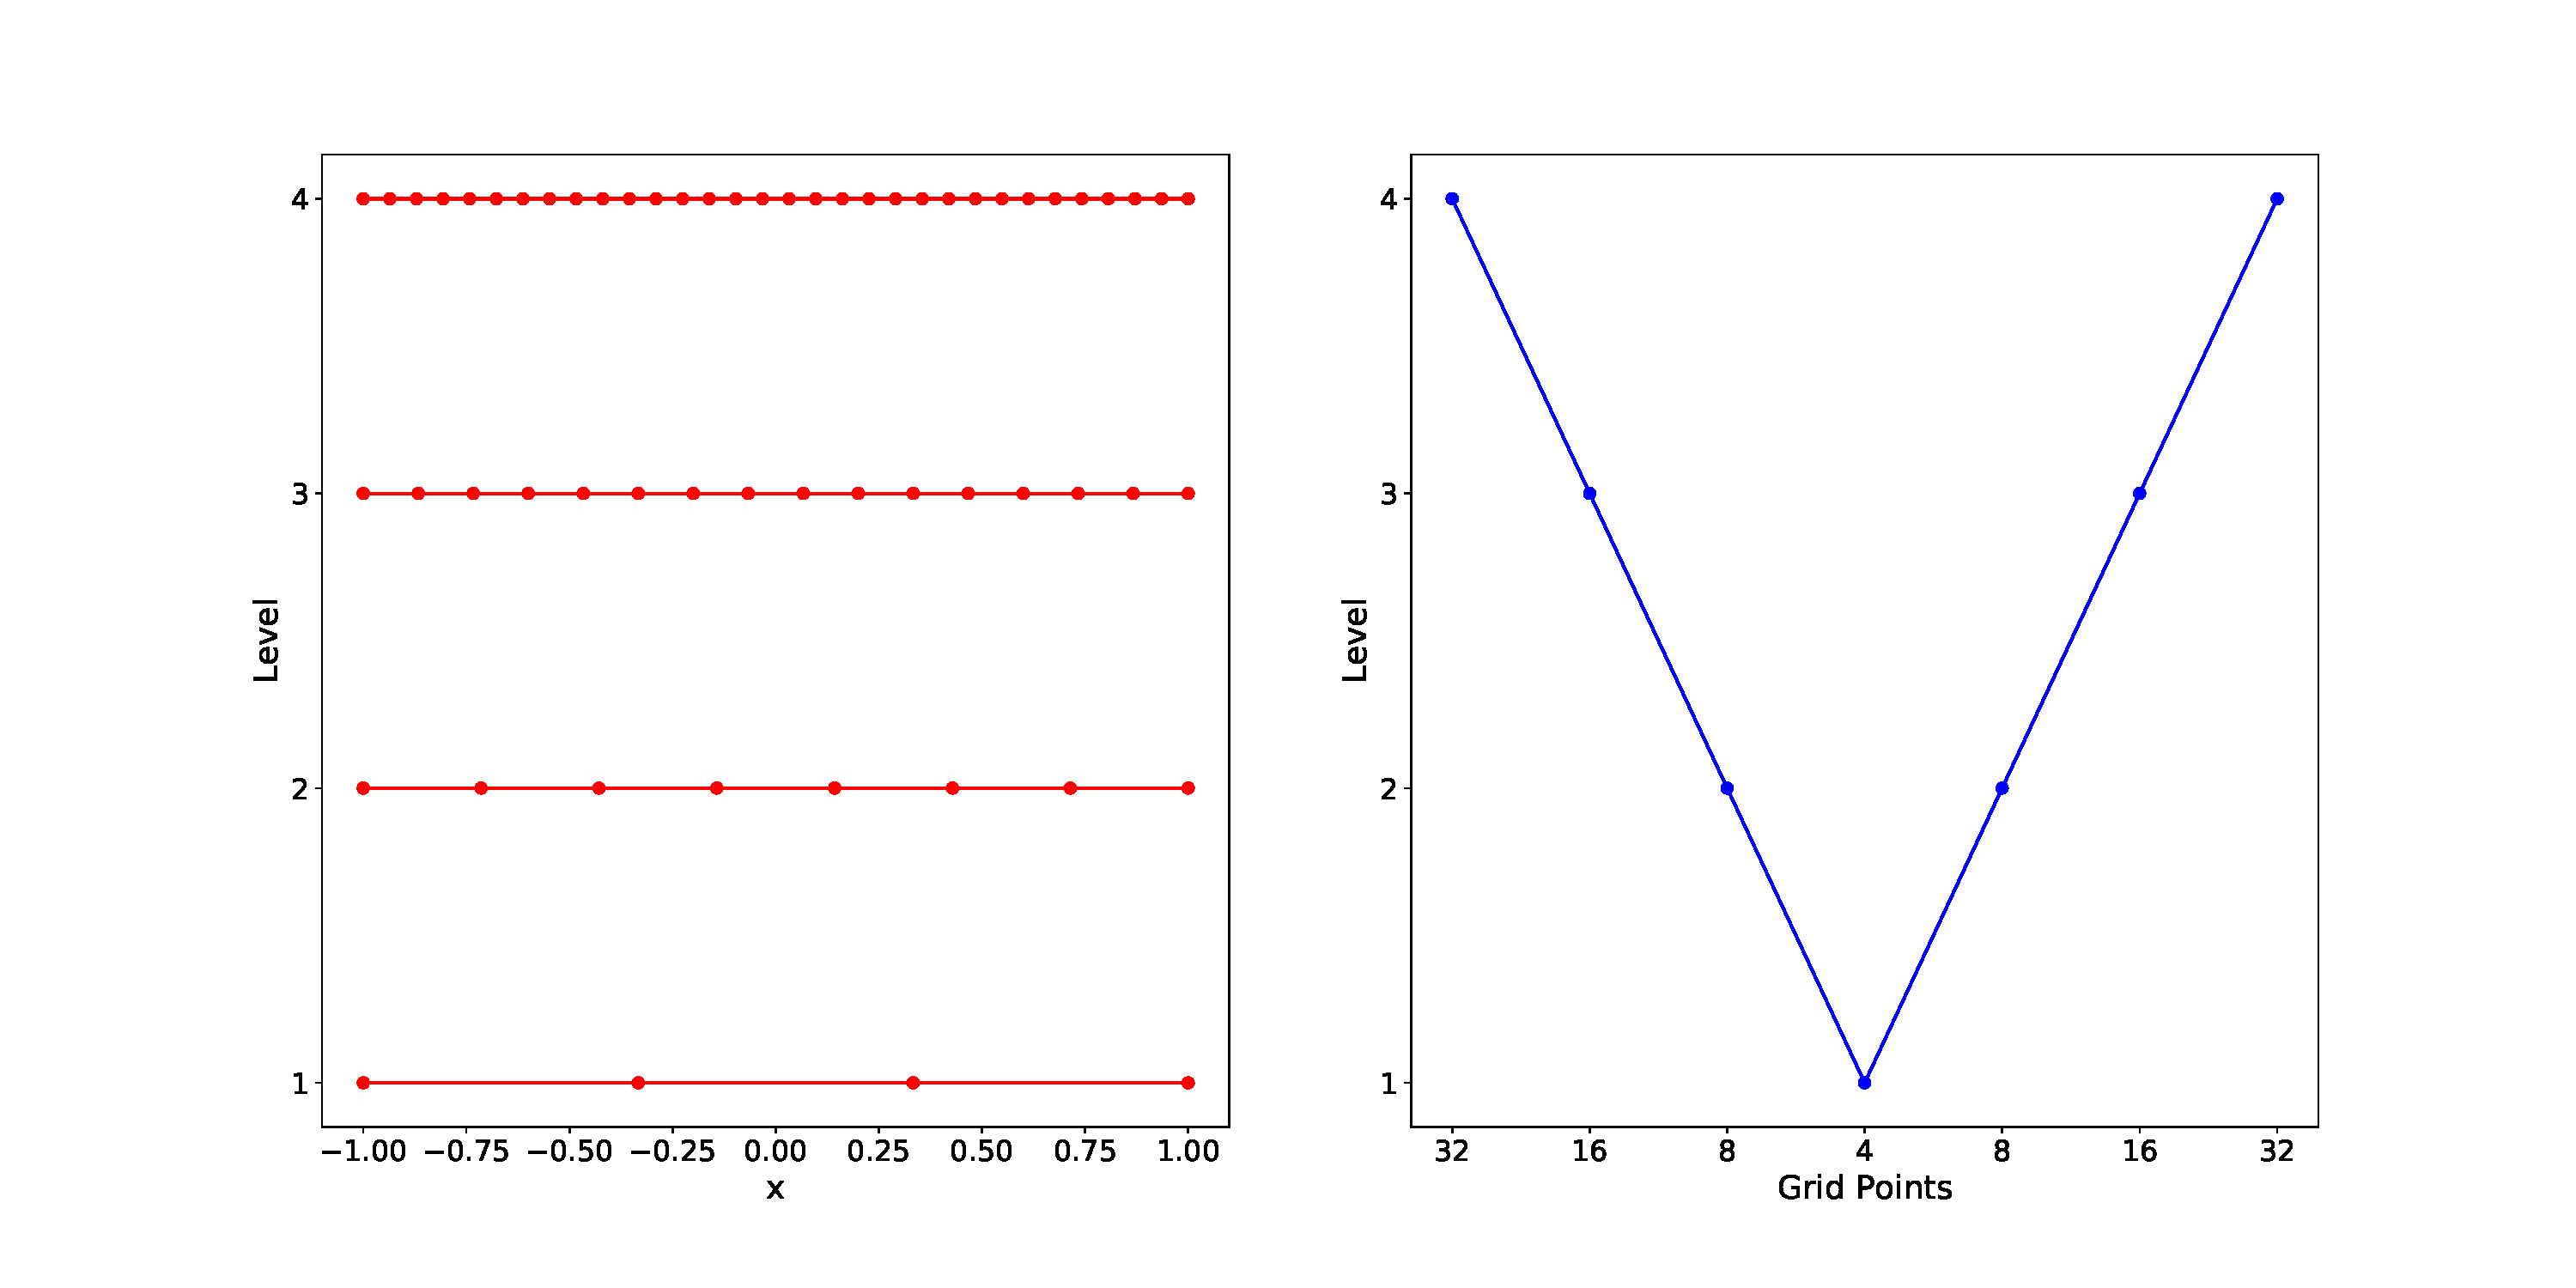
\includegraphics[width=0.8\columnwidth]{figures/multigrid.pdf}
    \caption{The 1D Multigrid Method. Starting with the finest grid, perform a few iterations of an iterative method. This is called relaxing the solution. Then project onto a coarser grid, and relax again. Do this down the levels in the grid to a desired precision. Once the solution is converged to on the coarsest level, interpolate back up the levels to obtain the solution on the finest level.}
    \label{fig:multigrid}
\end{figure}

In what is called the ``full multigrid" method, the process starts on the coarsest level instead of the finest. The solution is relaxed on this level, and then interpolated down onto a finer mesh. The interpolated solution is used as an initial guess for solving the problem on the finer mesh. The relaxed solution on a coarser grid is often an ideal initial guess for the problem on the finer mesh, resulting in quick convergence on that level.

The multigrid method allows one to accelerate an iterative solver. Multigrid methods are very effective as pre-conditioners for iterative methods. This is the general pattern of hierarchical methods: the ability to use classical iterative and direct methods on smaller grids where they perform well, and then ``scale" them up to larger problem sizes.

% \subsubsubsection{Nested Dissection}
% \label{subsub:nested-dissection}

{\bf Nested Dissection}
The nested dissection method formulated by George in \citep{george1973nested} is a direct method that builds upon Gaussian elimination for problems on a grid. It is also the basis for forming what is called the multifrontal method \citep{liu1992multifrontal, davis2004algorithm}. By taking advantage of the ordering of points on a grid, one can permute $\textbf{A}$ to first eliminate points that split the mesh into two disconnected meshes. This permutation takes the form of $\textbf{P}^* \textbf{A} \textbf{P}$, where the goal is to form $\textbf{P}$ to reorganize $\textbf{A}$ in a way that eliminates points in an efficient manner.

To detail nested dissection better, consider an $N \times N$ mesh such as a finite difference mesh discussed in Section \ref{subsub:finite-difference}. Assume that the initial ordering of points corresponds to an index set that iterates over the points in the mesh row-by-row. Now, the idea of nested dissection is to reorganize the points such that we first eliminate points down the middle of the mesh (i.e. the points at $x = 0$ in the first plot of Figure \ref{fig:discretization_methods}). Once these points are solved for, it splits the mesh into two equally sized pieces that are disconnected. Each of the disconnected meshes now are smaller, and thus easier to solve. This idea of splitting the mesh into disconnected pieces by first eliminating points along an interface can be recursively applied to each split. This means that after dividing the mesh into two, one can divide those two meshes into four meshes, and so on. Recursive splitting is a common characteristic in hierarchical methods.

Nested dissection was first introduced by George in \citep{george1973nested}, and further generalized by Lipton et al. in \citep{lipton1979generalized}. Martinsson has a tutorial on nested dissection in \citep{martinsson2019fast}. In fact, nested dissection served as motivation for another hierarchical method proposed by Martinsson and Gillman called the Hierarchical Poincaré-Steklov method.

% \subsubsubsection{The Hierarchical Poincaré-Steklov Method}
% \label{subsub:hps-method}

{\bf The Hierarchical Poincaré-Steklov Method}
Gillman and Martinsson introduce the Hierarchical Poincaré-Steklov (HPS) method \citep{martinsson2004fast, MARTINSSON2013460, gillman2014direct, martinsson2015hierarchical}. It is a direct solver for elliptic PDEs that is based on a binary tree of rectangular patches where the solution operator to $\textbf{A}$ is built by recursively merging child patches. Like direct methods, the HPS method involves a factorization step and a solve step. Unlike other direct methods, however, the HPS method is considered a matrix-free method as there is no requirement to form the system matrix $\textbf{A}$.

The HPS method starts with on a logically Cartesian domain, and recursively divides the domain in half. This creates a binary tree of patches as shown in Figure \ref{fig:solve}. Once the domain has been decomposed into this tree of patches, two operators are defined on the lowest level, called the leaf level. These operators are the solution operator $\textbf{S}$ and Dirichlet-to-Neumann (DtN) operator $\textbf{T}$. The solution operator maps boundary data to solution data on the interior of the patch (i.e. solves the local boundary value problem), and the DtN operator maps Dirichlet data on the boundary to Neumann data on the boundary. These operators can be formed using any elliptic PDE solver, including fast solvers like spectral methods. After forming these operators, the next step is to recursively merge each sibling patch up the tree. the merge step is demonstrated in Figure \ref{fig:merge}. This results in a global solution operator that can be stored and used multiple times (at different time steps or with varying boundary conditions, etc.), and is similar to a direct method matrix factorization. The final step is applying the solution operator to each level down the tree to obtain the solution everywhere in the domain. This step is just a matrix-vector multiplication and is very fast.

Similar to other direct methods, the HPS method forms an in-memory solution operator that can be applied to several right-hand side vectors. This property makes it ideal for problems where several elliptic solves are necessary. While most iterative methods have better asymptotic performance than other direct methods, the HPS method can be accelerated using hierarchically block separable (HBS) matrix algebra to achieve near linear asymptotic performance \citep{gillman2014direct}.

The \gls{hps} method has been applied to solve 3D elliptic \gls{pdes} \citep{hao2016direct}, has been coupled with the spectral element method \citep{fortunato2020ultraspherical}, and implemented on adaptive meshes \citep{babb2018accelerated, geldermans2019adaptive,chipman2024fast}. Recently, the \gls{hps} method has also been implemented in parallel, targeting shared-memory machines \citep{beams2020parallel}, distributed-memory machines \citep{yesypenko2022parallel}, and \gls{gpu} devices \citep{yesypenko2022gpu}. More details on the \gls{hps} method can be found in Chapters 19--27 of \citep{martinsson2019fast} and a tutorial on the \gls{hps} method can be found in \citep{martinsson2015hierarchical}.

\begin{figure}
    \centering
    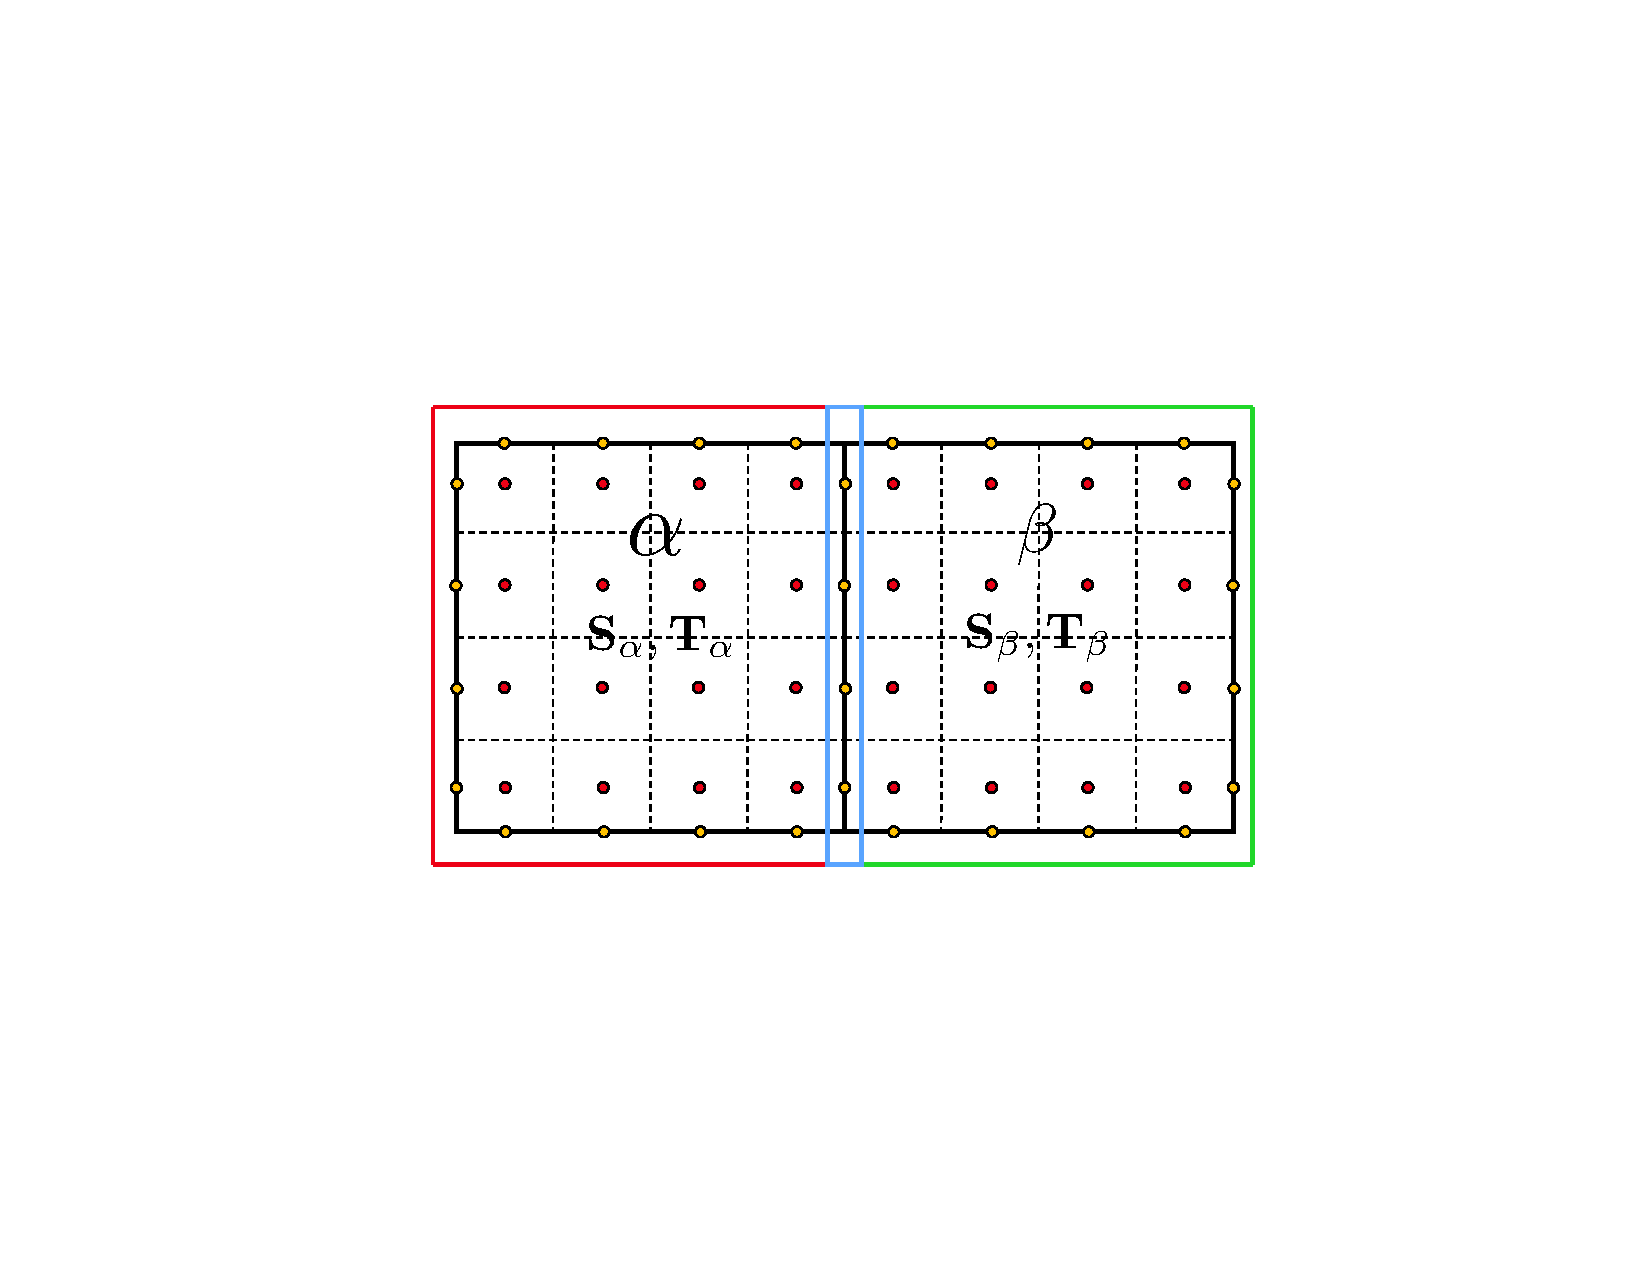
\includegraphics[width=0.7\columnwidth]{figures/merge_figure.pdf}
    \caption{HPS Merge Operation. The merged patch $\Omega_{\tau}$ is the union of children $\Omega_{\alpha}$ and $\Omega_{\beta}$, i.e. $\Omega_{\tau} = \Omega_{\alpha} \cup \Omega_{\beta}$. Red, green, and blue nodes correspond to index sets $\textbf{I}_1$, $\textbf{I}_2$, and $\textbf{I}_3$, respectively. The merge operation eliminates the nodes on the interface of the children patches.}
    \label{fig:merge}
\end{figure}

\begin{figure}
    \centering
    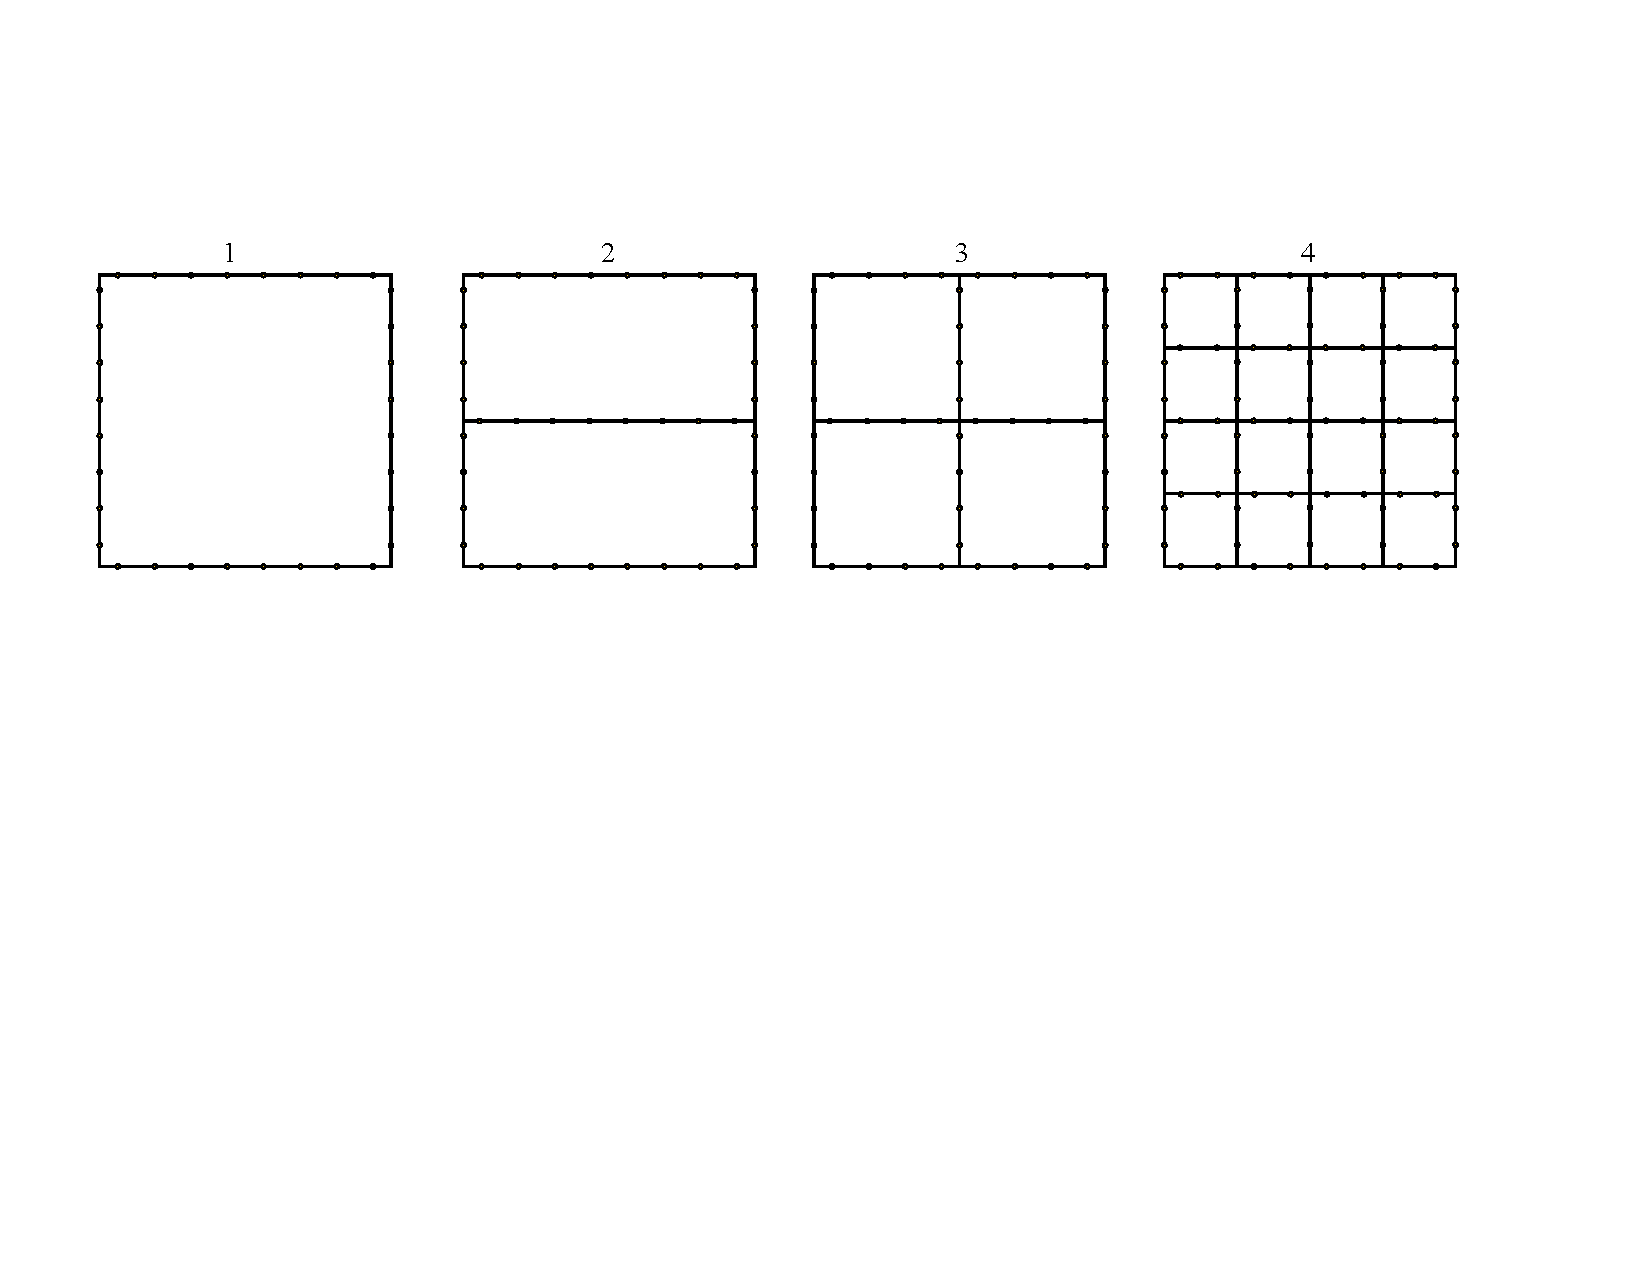
\includegraphics[width=\columnwidth]{figures/solve_figure.pdf}
    \caption{HPS Solve Stage. Once $\textbf{S}_0$ is formed, apply it to the top level Dirichlet data to get boundary (and solution) data on the interface of the children. Apply the patch solution operator down the tree until each leaf has it's local boundary information. Then apply the solution operator to get the solution data in the interior of each leaf.}
    \label{fig:solve}
\end{figure}


% \subsection{Fast Solvers for Elliptic PDEs}

% The linear systems formed by discretizations of elliptic \gls{pdes} are sparse and banded. Numerical linear algebra techniques that take advantage of this structure are ideal. Efficient solvers have been developed for uniform Cartesian meshes, such as the Unsymmetrical Multifrontal method implemented in the UMFPACK code \citep{davis2004algorithm} or the Cyclic Reduction method \citep{swarztrauber1974direct} as implemented in the FISHPACK library \citep{swarztrauber1999fishpack,adams2016fishpack90}.

% \citet{gillman2014direct} describe a direct solver for elliptic problems on a binary tree structure. The goal is to build up a factorization by successively merging subdomains via a class of Poincar\'e-Steklov operators \citep{quarteroni1991theory} called \gls{d2n} operators. It is a domain decomposition method that was originally inspired by the partitioning scheme of nested dissection \citep{george1973nested,lipton1979generalized}. This approach does not require any matrix assembly on the composite mesh and can be used with any uniform grid solver at the leaf level. In their original work, \citet{gillman2014direct} use high-order spectral collocation methods and low-rank optimization to achieve $\mathcal O(N)$ factorization complexity. This method has come to be known as the \gls{hps} method \citep{martinsson2015hierarchical}. The \gls{hps} method has been applied to solve 3D elliptic \gls{pdes} \citep{hao2016direct}, has been coupled with the spectral element method \citep{fortunato2020ultraspherical}, and implemented on adaptive meshes \citep{babb2018accelerated, geldermans2019adaptive,chipman2024fast}. Recently, the \gls{hps} method has also been implemented in parallel, targeting shared-memory machines \citep{beams2020parallel}, distributed-memory machines \citep{yesypenko2022parallel}, and \gls{gpu} devices \citep{yesypenko2022gpu}. More details on the \gls{hps} method can be found in Chapters 19--27 of \citep{martinsson2019fast} and a tutorial on the \gls{hps} method can be found in \citep{martinsson2015hierarchical}. A more in-depth description of the \gls{hps} method outlined by \citet{gillman2014direct} will be provided in \refsec{subsub:hps-method}.

% \damyn{[Direct vs. iterative solvers discussion.]}

\subsection{Parallelism and Software}

Parallel linear solvers using iterative or direct methods have been successfully developed and implemented. Parallel iterative methods include GMRES \citep{saad1986gmres}, the conjugate gradient method \citep{hestenes1952methods}, the \gls{amg} method \citep{yang2002boomeramg}, and the \gls{gmg} method \citep{sundar2012parallel} (with a good overview provided by \citet{chow2006survey}). Parallel direct methods include matrix factorization methods like LU-factorization, Cholesky factorization and the spectral value decomposition \citep{donfack2015survey, demmel1999asynchronous, gupta1997highly}.

% References for parallel methods?

Several, large-scale and open-source codes currently exist to solve linear systems formed from elliptic PDEs. The hypre library \citep{falgout2002hypre} features scalable preconditioners for parallel multigrid methods. The SuperLU library \citep{li2005superlu} is a general purpose library for solving sparse linear systems using direct methods. Additional codes like PETSc \citep{anl2023petsc}, FLASH-X \citep{dubey2022flash}, and AMReX \citep{zhang2019amrex}, contain iterative and direct solvers that also work with \gls{amr}. The ForestClaw code \citep{calhoun2017forestclaw} coupled with the ThunderEgg repository \citep{aiton2022thunderegg} implements hyperbolic and elliptic solvers for finite volume meshes on adaptively refined quadtrees and octrees provided from \pforest. \pforest\ \citep{burstedde2011p4est,burstedde2020parallel} is a highly scalable AMR code that provides quadtree and octree data structures for users to build on top of. The EllipticForest library \citep{chipman2024ellipticforest} contains an implementation of the quadtree-adaptive HPS method, including the parallel algorithms outlined in this paper. Another code of interest is the ButterflyPACK library \citep{liu2018butterflypack} that solves large-scale dense systems with off-diagonal, low-rank structure like the matrices formed in the HPS method.